\section{Acceleration Constraints}
In order to achieve the goal of minimising the time that the DoodleBot takes to complete a curve, the acceleration limits must be considered. These limits are the main design parameter that has a direct impact on the completion time for all curves. Figure \ref{fig:maxAccel} demonstrates the effect that increasing the acceleration limits has on the completion time for a given trajectory. It becomes clear that it is desirous to increase the acceleration limits as far as possible. However there are physical limits which degrade performance past certain thresholds.

\begin{figure}[htbp]  
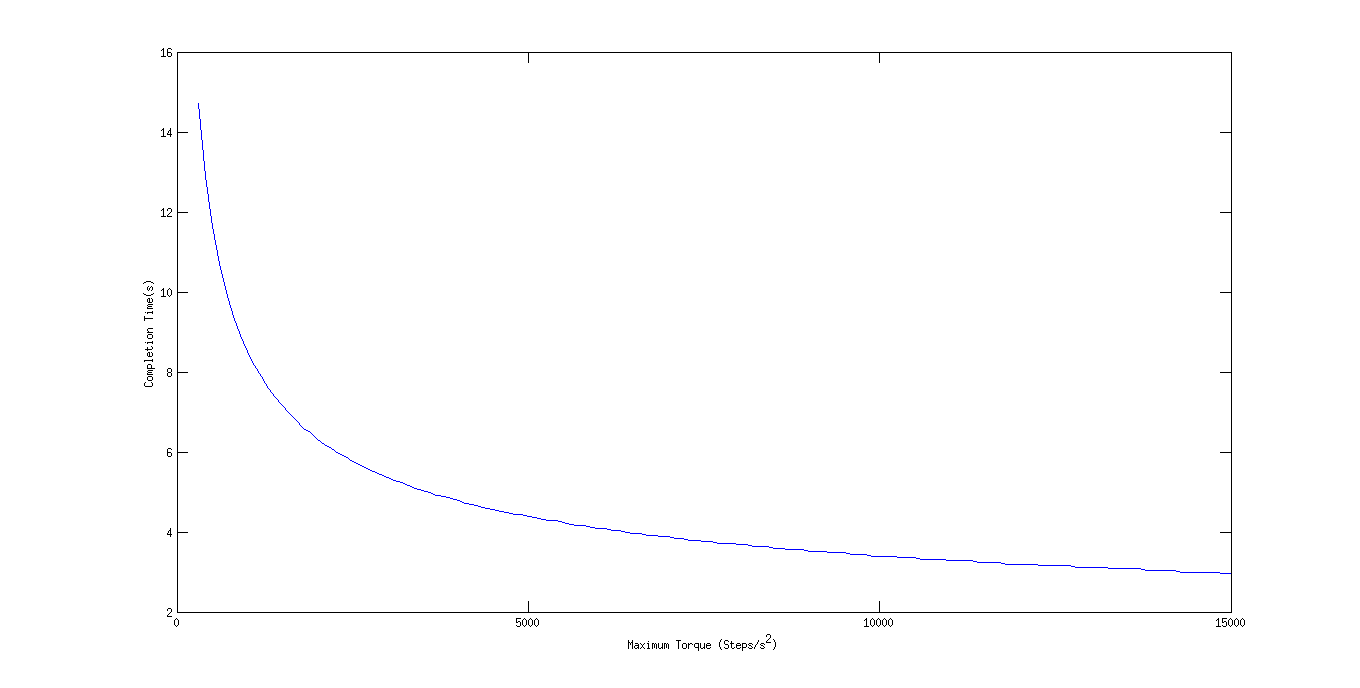
\includegraphics[width=\textwidth]{figures/performance/maxTorque.png}
\caption[Trajectory completion time against maximum acceleration limits]{Trajectory completion time against maximum acceleration limits
\label{fig:maxAccel}}
\end{figure}  	

The plant model derived for the DoodleBot allowed us to consider that for given acceleration limits the plant maps input to output perfectly. This allows us to give commands in open loop without fear of inaccuracy as long as we can guarantee that the acceleration limits will not be exceeded. As the plant is worked closer and closer to its limitations the perfect mapping of input to output begins to break down, resulting in unavoidable inaccuracy. There are two types of behaviour which can occur whilst close to the acceleration limits. 

The first is a catastrophic synchronisation failure between the step commands and the movements of the stepper motor. If the motor falls out of sync, step inputs essentially become random perturbations on the motor spindle. This means that the motor gains no net torque from the power input into the stepper coils, as the direction that the spindle is pulled is no longer in necessarily in the direction of desired travel due to the lack of synchronicity. The step commands come faster and faster and the motor spindle will simply vibrate in place, as the spindle cannot hope to accelerate to catch back up to the step rate. This type of failure is obvious and results in a complete failure to match the desired curve.

The second type of failure is a missed step, which occurs when a transient or other load causes the motor to fail to achieve the correct position by the time that the controller progresses to the next step. For a few subsequent steps, the motor continues under its own momentum with the step input of the controller assisting or hindering its progress at random. If the motor does not completely fall out of sync, the pulses will eventually realign themselves with the motor and the motor will continue without a total failure. These missed steps are not detected by the controller and will become a permanent offset for the rest of the motor's movement until there is a complete readjustment of the mechanism. Indeed these missed steps happen over a matter of milliseconds, so it is hard for human operators to tell when this kind of error occurs.

Higher accelerations also amplify the effect of the sample time error found in Section ~\ref{ch:performance-sampletime}.

A range of curves run at differing acceleration limits can be seen in Figure \ref{fig:accelLimits}.
	
\begin{figure}[htbp]  

\includegraphics[width=\textwidth]{figures/performance/accelLimits.png}
\caption[Comparison of differing acceleration constraints]{A comparison of the results of differing acceleration constraints. From top left to bottom right; 1) $1000\text{ steps}/s^2$ 2) $3000\text{ steps}/s^2$ 3) $5000\text{ steps}/s^2$ 4) $15000\text{ steps}/s^2$
\label{fig:accelLimits}}
\end{figure}  	

Measuring the accuracy of differing acceleration limits and attempting to notice the effect of step skipping is a complicated by the fact that lower acceleration limits result in a longer traversal time. This longer traversal time means that the velocity profile sampling has a higher equivalent density along the surface of the same curve. This results in better performance when the curve is traversed at a slower rate. Thus efforts to measure the accuracy of the mechanism under different acceleration constraints can be confounded. The limits on acceleration also depend on various factors that can change with time such as; the total load on the armature, friction at points along the axis, voltage supply fluctuations and a myriad of other possibilities.

For this reason it is sound practice to leave a solid buffer between the maximum measured acceleration limits of the device and the constraints given to the optimisation algorithm in order to allow for robustness to error. For the DoodleBot, this level was set to be $1000\text{ steps}/s^2$ as a default, though good performance could be obtained at higher acceleration limits with calibration.
